\documentclass[svgnames]{beamer}


\mode<presentation>
{
  \usetheme[titleformat=smallcaps,numbering=fraction,progressbar=frametitle]{metropolis}
  \usecolortheme[light,accent=orange]{solarized}
  %\usecolortheme[named=Goldenrod]{structure}
  % or ...

  \setbeamercovered{transparent}
  % or whatever (possibly just delete it)
}


% \usepackage{mathtext}
\usepackage[utf8]{inputenc}
\usepackage[english,russian]{babel}
\usepackage{cmap}
\usepackage{amsmath}
\usepackage{booktabs}
\hypersetup{unicode=true}
\graphicspath{{images/}{slides/images}}


\title[QTA 07] % (optional, use only with long paper }
{Дистрибутивная семантика}

\subtitle
{Квантитативный анализ текста} % (optional)

\author%[Author, Another] % (optional, use only with lots of authors)
{Кирилл Александрович Маслинский}
% - Use the \inst{?} command only if the authors have different
%   affiliation.

\institute%[Universities of Somewhere and Elsewhere] % (optional, but mostly needed)
{ЕУСПб}
% - Use the \inst command only if there are several affiliations.
% - Keep it simple, no one is interested in your street address.

\date%[Short Occasion] % (optional)
{18.04.2022 / 07}

\subject{natural language processing, text mining}
% This is only inserted into the PDF information catalog. Can be left
% out. 



% If you have a file called "university-logo-filename.xxx", where xxx
% is a graphic format that can be processed by latex or pdflatex,
% resp., then you can add a logo as follows:

% \pgfdeclareimage[height=0.5cm]{university-logo}{university-logo-filename}
% \logo{\pgfuseimage{university-logo}}

% Delete this, if you do not want the table of contents to pop up at
% the beginning of each subsection:

\newcommand{\plate}[1]{\begingroup\setbeamercolor{background canvas}{bg=Beige}
  % \begin{frame}<beamer>{Outline}
  %   \tableofcontents[sectionstyle=show/hide,subsectionstyle=show/shaded/hide]
  % \end{frame}
  \begin{frame}[plain]
  \vfill
  \centering
  \begin{beamercolorbox}[sep=8pt,center,shadow=true,rounded=true]{title}
    \usebeamerfont{title}#1\par%
  \end{beamercolorbox}
  \vfill
  \end{frame}
  \endgroup
}

% \AtBeginSection[]
% {
%   \begin{frame}<beamer>[plain]{План}
%     \tableofcontents[sectionstyle=shaded,subsectionstyle=hide]
%   \end{frame}
% }

% \AtBeginSubsection[]
% {
%   \begin{frame}<beamer>[plain]{План}
%     \tableofcontents[sectionstyle=shaded,subsectionstyle=show]
%   \end{frame}
% }

\newcommand{\tb}[1]{\colorbox{yellow}{#1}\space}
\newcommand{\Sp}[1]{\colorbox{green}{#1}\space}
\newcommand{\Sn}[1]{\colorbox{red}{#1}\space}


\begin{document}

\begin{frame}
  \titlepage
\end{frame}

\section{Дистрибутивная гипотеза}

\plate{co-occur | collocates}

\begin{frame}
  \frametitle{Дистрибутивная гипотеза: Firth}
  \begin{block}{Firth 1935}
    the complete meaning of a word is always contextual, and no study
    of meaning apart from context can be taken seriously
  \end{block}
  \begin{block}{Firth 1957}
    You shall know a word by the company it keeps
  \end{block}
\end{frame}

\begin{frame}
  \frametitle{Дистрибутивная гипотеза Зеллига Харриса}
  %% Пример из Зеллига Харриса
    \begin{block}{Harris 1954}
    The fact that, for example, \alert{not every adjectives occurs with every noun} can be used as
    a \alert{measure of meaning difference}. For it is not merely that different members of the
    one class have different selections of members of the other class with which they are
    actually found. More than that: if we consider words or morphemes A and B to
    be more different than A and C, then we will often find that the distributions of A and
    B are more different than the distributions of A and C. In other words, \alert{difference in
    meaning correlates with difference in distribution}.
  \end{block}
\end{frame}

\section{Иллюстрация: дистрибутивная гипотеза в действии}

\begin{frame}
  \frametitle{Корпус дня: ДетКорпус}
  \begin{columns}
    \column{.5\textwidth}
    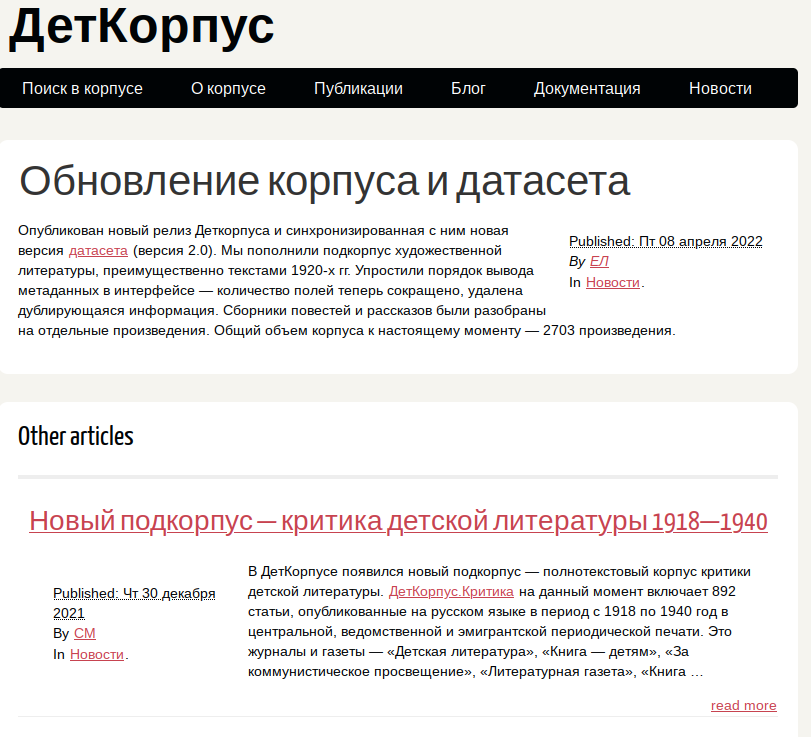
\includegraphics[width=\textwidth]{detcorpus.png}
    \column{.5\textwidth}
    \begin{itemize}
    \item Корпус прозы для детей и юношества на русском языке
    \item Период: 1900—2019
    \item 2573 произведений, 73 млн слов
    \item Поисковый интерфейс: \href{http://detcorpus.ru}{http://detcorpus.ru}
    \end{itemize}
  \end{columns}
\end{frame}

\begin{frame}
  \frametitle{Значение и сочетаемость}
  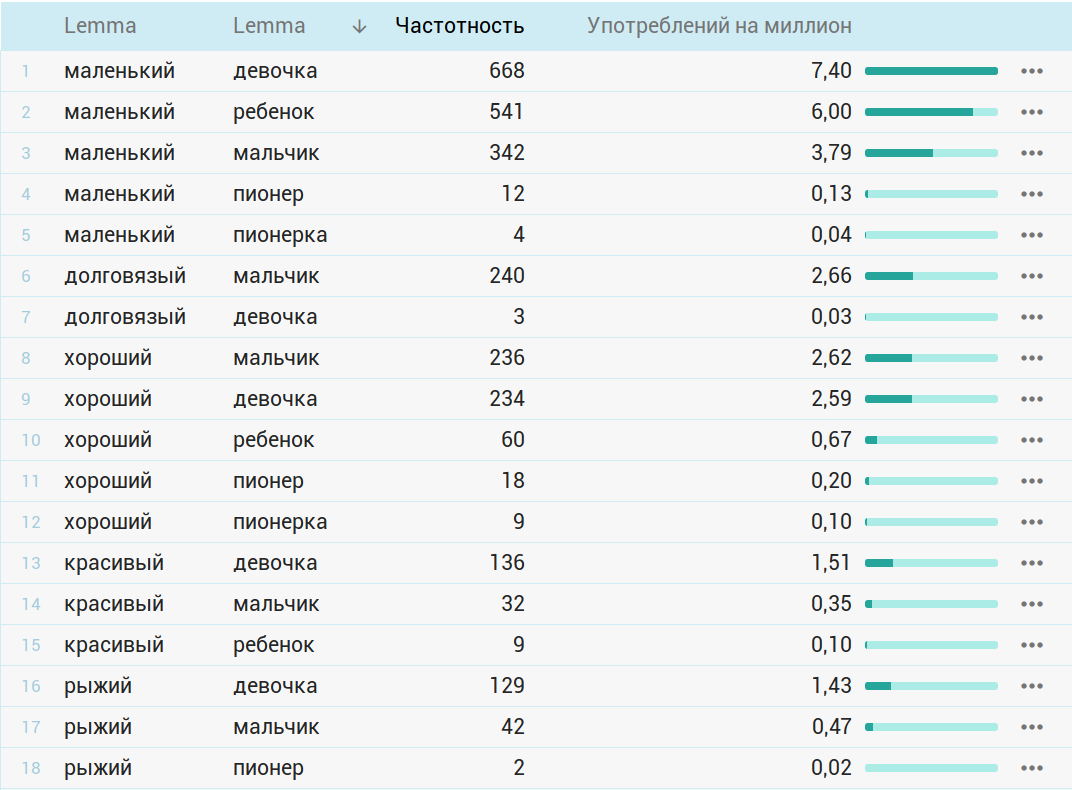
\includegraphics[width=.9\textwidth]{adjectives.png}\footnote{Статистика
  из ДетКорпуса: \href{http://detcorpus.ru}{http://detcorpus.ru}}
\end{frame}

\begin{frame}
  \frametitle{Контекстные вектора}
  \footnotesize
  \begin{tabular}[t]{lrrrrrr}
\toprule
  & воспитанный & худенький & чужой & долговязый & младший & юный\\
\midrule
девочка & 85 & 56 & 38 & 3 & 25 & 3\\
мальчик & 24 & 40 & 21 & 240 & 52 & 1\\
пионер & 0 & 0 & 1 & 0 & 3 & 120\\
пионерка & 0 & 0 & 0 & 0 & 1 & 1\\
ребенок & 15 & 3 & 107 & 0 & 32 & 0\\
\bottomrule
\end{tabular}
\end{frame}

\begin{frame}
  \frametitle{Дистрибуция в пространстве}
  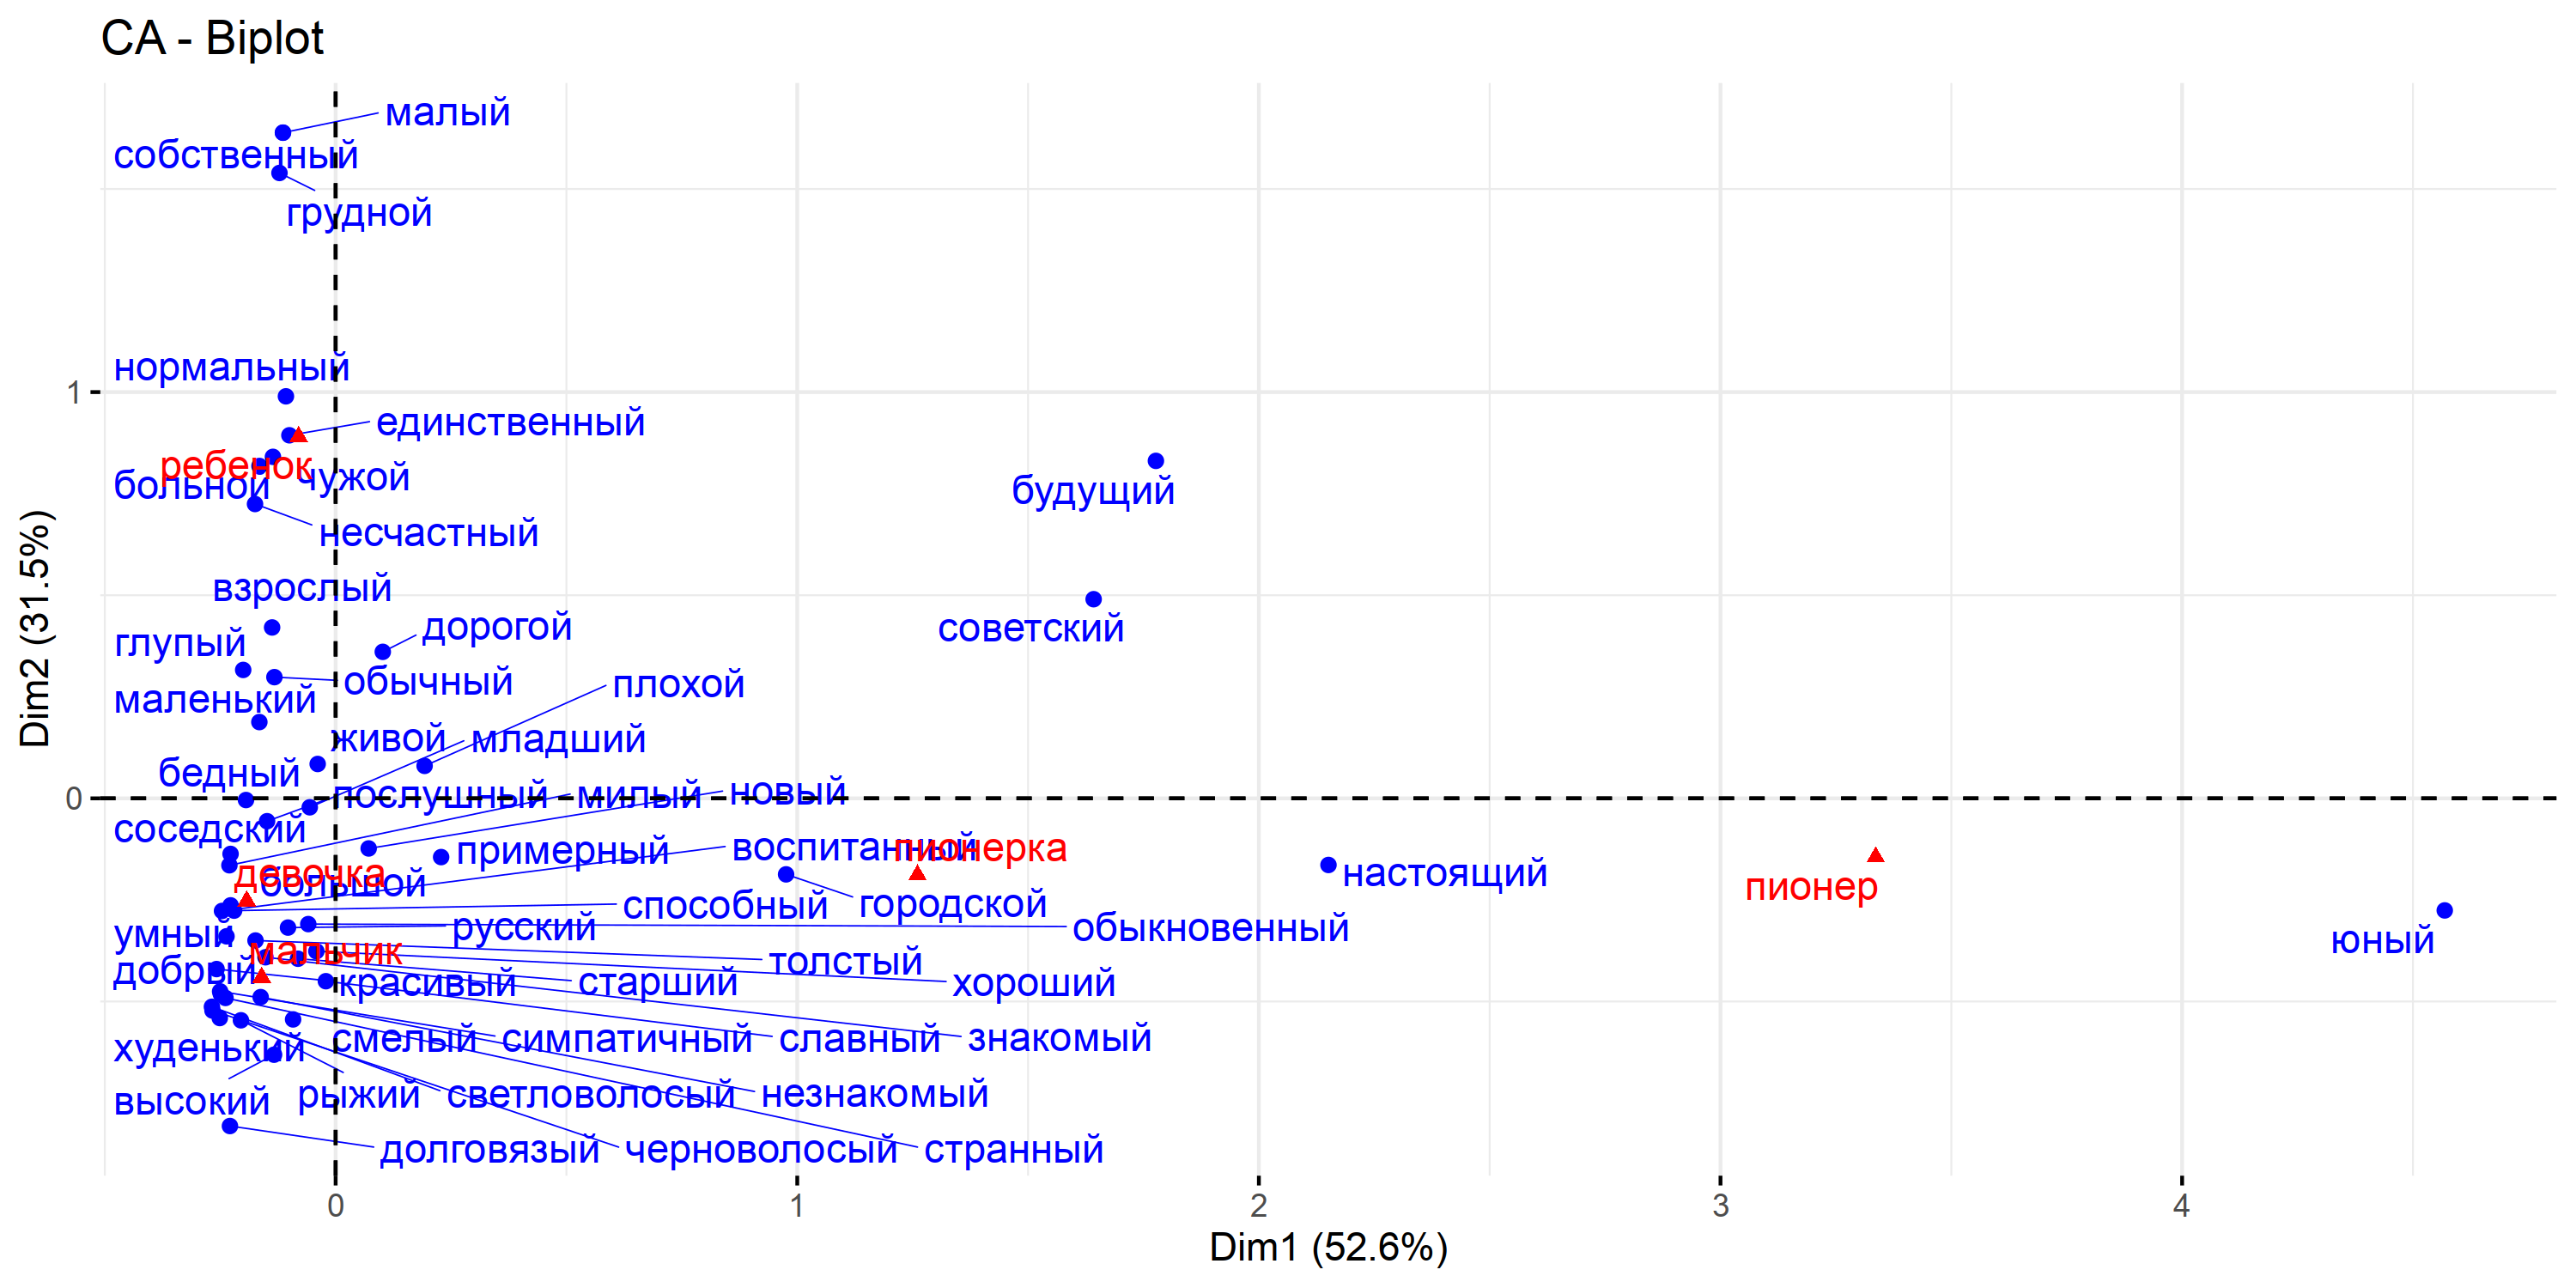
\includegraphics[width=\textwidth]{deti.png}\footnote{Анализ
    соответствий (Correspondence Analysis), выполненный по данным о
    распределении 50 самых частотных прилагательных в контексте слов
    ребенок/мальчик/девочка/пионер/пионерка, по данным ДетКорпуса}
\end{frame}

\section{Разновидности дистрибутивного анализа}

\begin{frame}
  \frametitle{Дистрибутивные данные}
  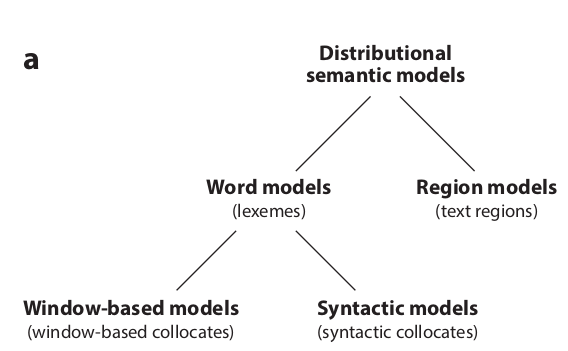
\includegraphics[width=\textwidth]{dsm-types}
\end{frame}

\begin{frame}
  \frametitle{Контекстное окно}
  \includegraphics<1>[width=\textwidth]{deti-kwic.png}
  \includegraphics<2>[width=\textwidth]{wider-context.png}
\end{frame}

\section{Методы снижения размерности}

\begin{frame}
  \frametitle{Метод главных компонент}
  \centering
  \LARGE
  \href{http://setosa.io/ev/principal-component-analysis/}{PCA — Principal component analysis}
\end{frame}

\begin{frame}
  \frametitle{Singular Value Decomposition}
  \includegraphics<1>[width=.9\textwidth]{basic-svd}
  \includegraphics<2>[width=.9\textwidth]{svd-matrices}
  \begin{itemize}
  \item Truncated SVD: производит «сгущенную»
    матрицу, в которой связанные строки и столбцы частично объединены.
  \item Измерений (колонок) в результирующей матрице меньше, чем в
    исходной.
    % \item Эти измерения соответствуют осям наибольшей дисперсии.33`
  \item метод, родственный \textbf{анализу главных компонент} (PCA).
  \end{itemize}
\end{frame}

\section{Латентный семантический анализ (LSA)}

\begin{frame}
  \frametitle{LSA}
  Слова и документы — вектора в семантическом пространстве, измерения
  которого представляют собой «латентные» переменные.
  \begin{itemize}
  \item совместно встречающиеся слова проецируются на одни и те же измерения;
  \item вектор для документа — взвешенная сумма векторов входящих в него слов (центроид);
  \item в семантическом пространстве угол между векторами документов
    может быть малым, \alert{даже если в документах нет общих слов}.
  \end{itemize}
\end{frame}


\begin{frame}
  \frametitle{Применение LSA}
  Можно оценивать семантическую близость (сходство):
  \begin{itemize}
  \item слово—слово
  \item слово—документ
  \item документ—документ
  \item документ—слово
  \end{itemize}
  Характерные применения LSA:
  \begin{itemize}
  \item поиск документов, близких к запросу (killer feature для
    информационного поиска);
  \item выявление семантически близких слов (синонимов);
  \item оценка связности текста (семантической близости соседних абзацев);
  \item извлечение ключевых слов текста.
  \end{itemize}
\end{frame}


\end{document}
